\chapter{Background}
\label{ch:Foundation}
\begin{figure*}
    %
    \centering
     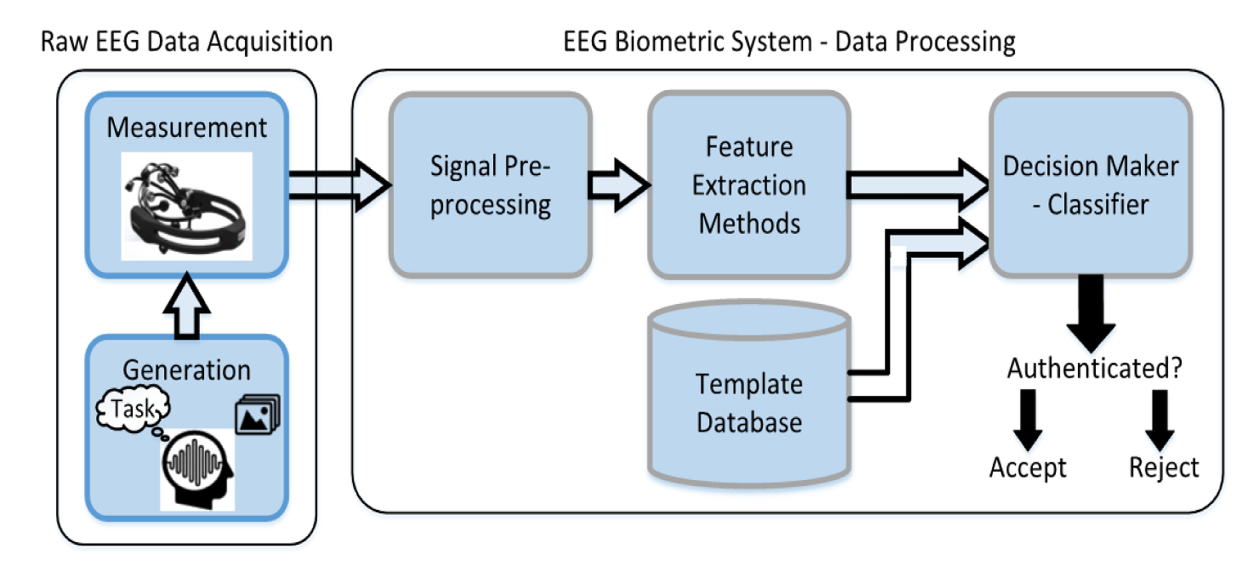
\includegraphics[width=0.72\textwidth]{figures/Authentication pipeline.png}   
    %
    
    %\caption{SMC Learning Algorithm}
    \caption{An authentication process based on EEG involves a sequence of essential stages, including data acquisition, data processing, and the classifier acting as the decision maker \cite{arias2023performance}}. 
    \label{fig: BrainInvaders}
    
    
\end{figure*}
\section{Background on EEG}
\label{sec:Background:Background on EEG}
Developing a direct interface for communication and control between human brains and computers has been a subject of contemplation within the scientific community for an extended period. Numerous research and development initiatives have been employed to actualize this concept, resulting in its emergence as a highly burgeoning field of scientific investigation in recent times \cite{clinical_trails}. This vast area of research has also led to the development of something now known as Brain-Computer Interface (BCI). BCI technologies have been widely utilized in the healthcare industry. These technologies have been applied in various tasks, including fatigue detection, assessment of sleep quality, and clinical applications such as detecting and predicting abnormal brain diseases. Examples of these diseases include seizure disorders, Parkinson's disease, Alzheimer's disease, and schizophrenia \cite{BCI_applications}.
\smallskip

BCI can be classified into three groups: invasive, partially invasive, and non-invasive \cite{girouard2009distinguishing}. The first two classifications of BCIs necessitate the surgical placement of sensors(electrodes) within the brain cortex to capture the minute currents produced due to cerebral responses. While it is true that invasive methods of BCI offer enhanced signal quality, the associated surgical risks and the need for long-term implantation of invasive devices negate any potential advantages derived from better signal quality. \cite{velasco2019bci}. 
%On the other hand, non-invasive technology utilizes external neuroimaging devices to record brain activities, consisting of functional near-infrared spectroscopy (fNIRS), functional magnetic resonance imaging (fMRI), and electroencephalography (EEG). Non-invasive EEG-based devices have been the most widely utilized modality for practical BCIs and clinical applications due to the relative improvements in signal quality, dependability, and mobility compared with alternative imaging techniques
In contrast, non-invasive technology involves external neuroimaging devices to capture brain processes. This includes functional near-infrared spectroscopy (fNIRS), functional magnetic resonance imaging (fMRI), and electroencephalography (EEG). Utilizing non-invasive devices based on EEG has been prevalent in practical BCIs and clinical applications \cite{BCI_applications}. This is mainly owing to the notable enhancements in signal quality, reliability, and portability compared to other imaging techniques. The proliferation of affordable and highly portable EEG equipment, exemplified by various consumer devices such as Neurosky\footnote{\url{https://neurosky.com/}}, has expanded the application of BCIs beyond the confines of the healthcare industry and into domains such as gaming \cite{van2012designing}. Research on brain biometrics has recently garnered a lot of attention in this area, which has been further encouraged by the limitations of using passwords to prove online identity \cite{arias2021inexpensive}.  


\section{Devices for EEG measurements}
\label{sec:Background:EEG Instruments and Data Acquisition}

\begin{figure}%
    \centering
    \subfloat[\centering Medical grade EEG headset from g.tec \cite{gtecGtecMedical}]{{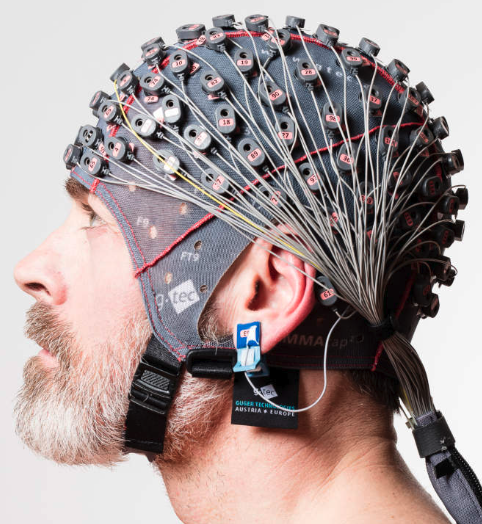
\includegraphics[width=5.5cm]{figures/Headset/G_tec_headset.png}}}%
    \qquad
    \subfloat[\centering EPOC/EPOC+ wearable headset \cite{emotivEPOCChannel}]{{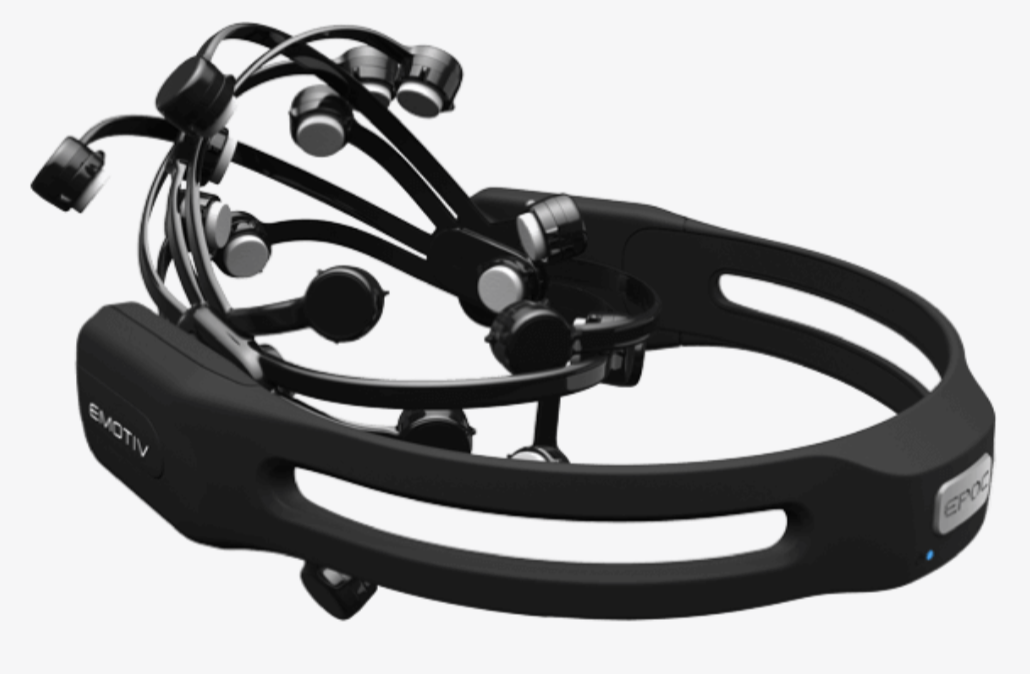
\includegraphics[width=6cm]{figures/Headset/Emotiv Comsumer Device.png} }}%
    \caption{In Figure (a), we can observe the g.GAMMAcap, which is among the frequently utilized medical-grade EEG headsets. Moving on to Figure (b), we see the EMOTIV EPOC+ device equipped with 14 EEG electrodes. }
    \label{fig: Headsets}%
\end{figure}
%\footnotetext{\url{https://www.gtec.at/}}
To acquire the EEG) signals, an EEG apparatus necessitates the inclusion of sensors capable of establishing conductive contact with the scalp. An amplifier that facilitates real-time filtering and common mode rejection, an analog-to-digital converter (A/D converter), and a personal computer (PC) to store the digitized data \cite{survey_brain_biometrics}. The EEG headset, which records the brain activity, includes sensors arranged according to the 10-20 or 10-10 system, which are international standards for consistent placement of electrodes, ensuring comparability across subjects and studies. The naming of the electrodes within these systems follows a specific convention that represents the brain region underneath (e.g., F for frontal, C for central) and an odd or even number indicating the hemisphere (odd for left, even for right) \cite{abhang2016introduction}. Frequently utilized EEG devices include the ActiveTwoSystem designed by Biosemi (Amsterdam, Netherlands)\footnote{\url{http://www.biosemi.com/}} and the g.GAMMAcap developed by G.Tech Medical Engineering GmbH\footnote{\url{https://www.gtec.at/}}. An example EEG headset from G.Tech is illustrated in Figure \ref{fig: Headsets} (a). These medical-grade EEG systems can support up to 256 channels, allowing for comprehensive data collection. This feature offers a benefit as it facilitates a greater extent of spatial coverage on the scalp, resulting in a more comprehensive dataset \cite{survey_brain_biometrics}.
\smallskip

Although medical-grade EEG devices are known for their ability to gather data of high quality, the considerable expense associated with these devices and the complexities needed in establishing the EEG connection pose notable obstacles. In response to these constraints, there has been a proliferation of cost-effective and user-accessible EEG devices in recent times, presenting viable substitutes. Instances of such devices include the ENOBIO developed by Neuroelectrics (Barcelona, Spain)\footnote{\url{https://www.neuroelectrics.com/}}, the EPOC/EPOC+ wearable neuroheadset designed by Emotiv Systems, Inc. (San Francisco, USA)\footnote{\url{https://www.emotiv.com/epoc/}}, along with the Muse headband crafted by InteraXon (Ontario, Canada)\footnote{\url{https://choosemuse.com/}}. An EPOC/EPOC+ wearable EEG headset equipped with 14 sensors is depicted in Figure \ref{fig: Headsets} (b). Consumer devices are cheaper than medical-grade EEG headsets and more friendly but have a poor signal-to-noise ratio \cite{survey_brain_biometrics}. 

%Examples of these are the ENOBIO developed by Neuroelectrics (Barcelona, Spain)\footnote{\url{https://www.neuroelectrics.com/}}, the EPOC/EPOC+ wearable neuroheadset developed by Emotiv Systems, Inc. (San Francisco, USA)\footnote{\url{https://www.emotiv.com/epoc/}}, and the MindWave wearable headset developed by NeuroSky, Inc. (San Jose, USA) and Muse headband developed by InteraXon (Ontario, Canada). 


%BCI can be classified into three groups: invasive, partially invasive, and non-invasive. The former two categories of BCI require surgically inserting electrodes into the brain cortex to record the small currents generated due to brain responses. BCI can be classified into three groups: invasive, partially invasive, and non-invasive. The former two categories of BCI require surgically inserting electrodes into the brain cortex to record the small currents generated due to brain responses. 
% \begin{itemize}
% \item For EEG acquisition, an EEG device must incorporate sensors that can establish a conductive connection with the scalp. This device also requires a bio amplifier for real-time filtering and common mode rejection, an A/D converter for digital translation, and a computer system for storing the converted data.
% \item The headset includes sensors arranged according to the 10-20 or 10-10 system, which are international standards for consistent placement of electrodes, ensuring comparability across subjects and studies. These systems provide comprehensive coverage, allowing for detailed EEG data collection.

% \item The naming of the electrodes within these systems follows a specific convention that represents the brain region underneath (e.g., 'F' for frontal, 'C' for central) and an odd or even number indicating the hemisphere (odd for left, even for right).

% \item The EEG headsets can be medical grade, such as ActiveTwoSystem by Biosemi (Amsterdam, Netherlands) or g.USBamp (G.Tech Medical Engineering GmbH. These medical-grade EEG devices can accommodate as many as 256 channels. One of the main disadvantages of using these devices is the longer preparation time. They are also costly.

% \item Recent advances in neurotechnology have led to the development of cheap and consumer-friendliness. Examples of these are the ENOBIO developed by Neuroelectrics (Barcelona, Spain)2, the EPOC/EPOC+ wearable neuroheadset developed by Emotiv Systems, Inc. (San Francisco, USA)3, and the MindWave wearable headset developed by NeuroSky, Inc. (San Jose, USA) and Muse headband developed by InteraXon (Ontario, Canada). Consumer devices are cheaper than medical-grade EEG headsets and more friendly but have a poor signal-to-noise ratio. 
% \end{itemize}

\section{Data Acquisition Procedures}
\label{sec:Background:Data Acquisition Procedures}
%EEG recording can be done 
% \begin{itemize}
%The firing of neurons in the brain is significantly influenced by the mental state of individuals, exhibiting a solid susceptibility to both external environmental stimuli and internal self-regulation. Hence, it is imperative to devise a specialized data collection paradigm to gather EEG signals \cite{zhang2021review}.
The activity of neurons in the brain is notably impacted by individuals' mental conditions, displaying a marked sensitivity to both external environmental triggers and internal self-control mechanisms. This necessitates the development of tailored data collection approaches for capturing EEG signals effectively \cite{zhang2021review}. 
EEG data acquisition often entails implementing meticulously planned EEG experiments, wherein subjects engage in a range of cognitive tasks or maintain a state of rest, with the option of having their eyes either open or closed \cite{survey_brain_biometrics}. 
\smallskip

Resting-related tasks are the simplest to accomplish. Typically, resting-state tasks involve recording brain activity when participants are in a calm, relaxed state and are not performing cognitive tasks. 
As a result, resting state protocols have been employed in many brainwave authentication studies such as \cite{nakanishi2009eeg, thomas2018eeg}. Paranjape \textit{et al.} \cite{paranjape2001electroencephalogram} suggested an EEG-based authentication system while subjects sit in a relaxed state with closed/open eyes task. The Autoregressive model (AR) was utilized for extracting the discriminant biological features, and a classification ACC of 80$\%$ was achieved. While the resting tasks offer simplicity in data collection, they are greatly influenced by the outside world, and it is not easy to ensure complete silence in a natural application environment \cite{zhang2021review}. 
\smallskip

In contrast to protocols for rest, protocols for cognitive activities are characterized by a higher degree of complexity. One category of cognitive protocols encompasses mental tasks. Mental tasks involve the subject imagining doing something specific (e.g., imagine moving their left and right hand or image closing or opening a fist), causing the associated EEG signals to appear \cite{survey_brain_biometrics}. Brigham and Kumar \cite{brigham2010subject} conducted a study involving the brain activity of six subjects who were instructed to imagine speaking two syllables, /ba/ and /ku/, at varying rhythms without any explicit guidance. Following a similar approach as observed in the study by Paranjape \textit{et al.} \cite{paranjape2001electroencephalogram}, the researchers in this study employed AR coefficients to extract features from the signals of each electrode. Employing the Support Vector Machine (SVM) classification model, their results demonstrated an impressive accuracy rate of 97.76$\%$. Mental tasks demonstrates suitability for people across various physical limitations and visual impairments, exhibiting a high degree of applicability \cite{zhang2021review}. Nevertheless, it is worth noting that motor imagery and mental tasks demand specialized training to generate proper responses, making them challenging to execute \cite{brigham2010subject}.
\smallskip

The other type of cognitive protocol is based on event-related potentials (ERP). ERPs are a particular type of evoked potentials, time-locked to brain variations that appear in reaction to external stimuli \cite{zhang2021review}. They are generally elicited by exposing subjects to external audio or visual stimuli. EPRs are influenced by the subject's knowledge, level of motivation, and cognitive capacities \cite{blackwood1990cognitive}, making them more likely to display distinctive, unique traits helpful for authentication. Mu \textit{et al.} \cite{mu2016eeg} introduced an innovative approach to ERPs by exposing participants to stimuli in the form of self-photos and non-self-photos. They utilized fuzzy entropy extracted from the EEG signals for the purpose of personal authentication. To classify these features, they employed Neural Networks (NN), yielding an impressive accuracy rate exceeding 87.3$\%$. One notable drawback of ERPs, in comparison to EEG, lies in the increased complexity of the elicitation methods associated with ERPs. EEG can be obtained without the need for any specific stimulation of the user, but ERPs can only be obtained when the user is subjected to a specific and carefully controlled kind of stimulation \cite{survey_brain_biometrics}.

%Mu \textit{et al.} \cite{EEG_table_EEG1} introduced a novel paradigm to elicit ERPs by presenting stimuli of self-photos and non-self-photos to the participants. To achieve personal authentication, the EEG signal's fuzzy entropy was determined and Neural Networks (NN) were employed for the classification, producing an ACC of more than 87.3$\%$.  

% \item The other type of cognitive protocol is based on event-related potentials (ERP). ERPs are a particular type of evoked potentials, time-locked to brain variations that appear in reaction to external stimuli. They are generally elicited by exposing subjects to external audio or visual stimuli. Some of the examples of ERP paradigm are P300 and N400. 

% \item ERPs present two significant advantages for biometric utilization over EEG. Firstly, EEG data captured without a concurrent cognitive task lacks specificity, meaning it doesn't provide clear insight into the participant's thoughts or mental state at the time of recording. In contrast, ERPs, which are time-locked to specific stimuli, precisely indicate the brain's response to that stimulation. 
% \end{itemize}

\section{EEG Pre-Processing Techniques}
\label{sec:Background:Common EEG Artifacts}
% \begin{itemize}

% \item 
After the EEG data is acquired, it is imperative to eliminate any noise intruding on the EEG signals to obtain clean and precise readings.
EEG signals can be corrupted by various artifacts, either of physiological or non-physiological nature. Physiological artifacts are non-EEG signals introduced by different biological activities such as heartbeat, muscle contractions, or eye movements. In contrast, non-physiological artifacts typically arise from the EEG acquisition system itself or external environmental factors, including electromagnetic fields from other electronic devices \cite{survey_brain_biometrics}. Following are some of the standard cleaning processes usually employed in EEG.   
\subsection{EEG Filtering}

\begin{figure*}
    \centering
    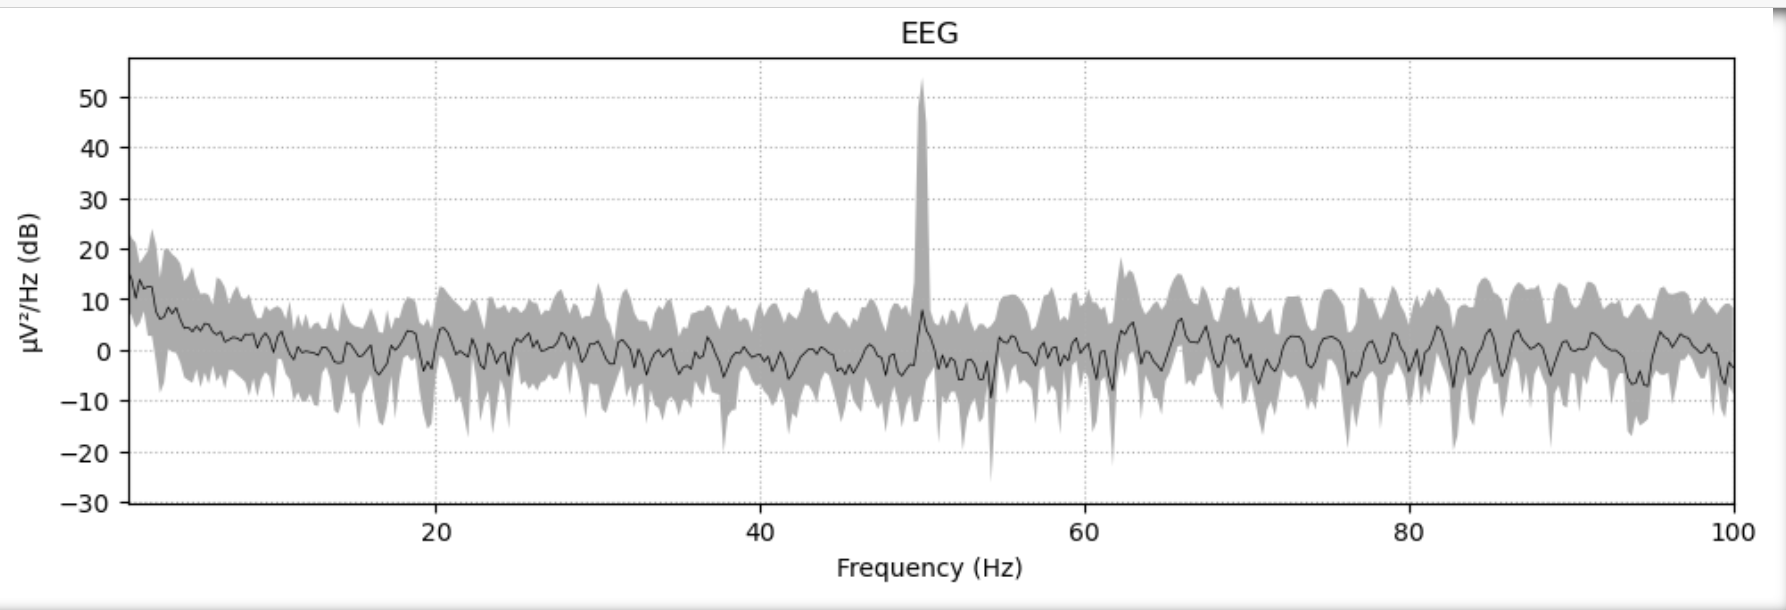
\includegraphics[width=\textwidth]{figures/background_psd_plot.png}  
    \caption{EEG signal strength against frequency, 0–100 Hz, showing 50 Hz line noise.}
    \label{fig: PSD of line noise}
\end{figure*}

As previously stated, EEG data is susceptible to interference from electrical appliances, leading to noise mostly at frequencies of 50 Hz in Europe (as depicted in Figure \ref{fig: PSD of line noise}) and 60 Hz in the USA. This phenomenon arises due to the prevailing power line frequencies in the corresponding geographical areas. Therefore, employing a notch filter, specifically a band-stop filter with a small stopband centered at 50 Hz or 60 Hz, is common practice to eliminate line noise effectively \cite{delorme2023eeg}. Other filtering methods include low pass filtering, which entails the elimination of higher frequencies, high pass filtering, which eliminates frequencies below a specific threshold while preserving high frequencies \cite{gonccales2021effects}; and bandpass filtering, which combines the above filtering techniques. 
The bandpass filter selectively keeps frequencies within the specified upper and lower bounds while eliminating frequencies that do not fall within this range. Furthermore, the Butterworth filter, known for its maximally flat magnitude in the passband, is widely used in pre-processing EEG data \cite{survey_brain_biometrics}.       
\subsection{Artifacts Rejection}
One often employed approach for mitigating physiological artifacts is discarding EEG data over a predefined threshold of EEG voltage \cite{jung2000removal}, such as 100$\mu$V since physiological artifacts generally exhibit significantly greater magnitudes in comparison to cerebral activity \cite{survey_brain_biometrics}. However, a more sophisticated method of rejecting artifacts is the peak-to-peak rejection method. This approach involves identifying and removing EEG segments that surpass a predetermined voltage range. This range is commonly determined by measuring the peak-to-peak amplitude, which is the difference between the highest positive and lowest negative deflections within a specific time frame \cite{luck2014introduction}. While the peak-to-peak rejection technique efficiently eliminates noisy signals, its application can inadvertently remove substantial valuable EEG data. This outcome is particularly possible when the method is not executed after meticulous assessment, as the amplitude of EEG signals can significantly differ based on experimental configurations and the characteristics of the utilized headsets.  

\subsection{Independent Component Analysis}
The Independent Component Analysis (ICA) is an innovative signal processing technique that enables the separation of sources that have been linearly mixed at the sensors. This separation is achieved by assuming simply the statistical independence of the sources \cite{vigario2000independent}. According to Hyv\"arinen \textit{et al.} \cite{hyvarinen1999fixed}, the ICA algorithm can be defined by the following equation.
\begin{equation}
S \cdot X=U
\end{equation}
where S is the unmixing matrix, X is the signal of EEG channels where each row corresponds to a sensor channel , and each column corresponds to a time point in the recorded signals and U represents the matrix of the estimated independent source signals. This method enables the segregation of EEG signals from noise and randomly mixed signals, contributing significantly to enhanced signal quality and analysis .  

%One often employed approach for mitigating physiological artifacts is discarding EEG data over a predefined threshold of EEG voltage \cite{jung2000removal}, such as 100$\mu$V since physiological artifacts generally exhibit significantly greater magnitudes in comparison to cerebral activity \cite{survey_brain_biometrics}. However, a more sophisticated method of rejecting artifacts is by employing peak to peak rejection. This approach involves identifying and removing EEG segments that surpass a predetermined voltage range. This range is commonly determined by measuring the peak-to-peak amplitude, which is the difference between the highest positive and lowest negative deflections within a specific time frame \cite{luck2014introduction}. 

% \item Physiological artifacts are particularly tricky as they emanate from the body's inherent processes. For instance, the electric fields produced during eye movements or blinks, heartbeats, muscle contractions, or even perspiration can introduce significant noise into the EEG signals. These artifacts often cause substantial voltage fluctuations that can easily exceed an amplitude of 100$\mu$V, thus, effectively masking the true EEG signal.

% \item Line noise is a prevalent artifact in EEG signals, generated by electronic equipment present during the EEG experiment. The circulating electrical current in the building's electrical system gives rise to an electromagnetic interference known as "line noise". This interference, detected by the EEG cables, has a frequency determined by the local power grid, usually 50 Hz in Europe and 60 Hz in the USA.
% \end{itemize}
\section{EEG Features}
\label{sec:Background:EEG Features}
The feature extraction technique is vital in EEG-based authentication, transforming pre-processed EEG signals into concise yet informative representations \cite{azlan2014feature}, facilitating accurate subject classification. EEG features can be organized into various domains, encompassing the time-domain (such as Auto Regressive Coefficients), the frequency-domain (like Power Spectral Density), and the time-frequency domain (including Wavelet Transform). The subsequent methods are frequently utilised for feature extraction in EEG-based authentication studies. 

\subsection{Auto Regressive Coefficients}
Autoregressive (AR) coefficients are a class of time-domain features frequently utilized in EEG-based authentication. %Autoregressive (AR) model is a stochastic process in which the output variable is linearly influenced by its previous values, together with an unpredictable stochastic term \cite{survey_brain_biometrics}. 
The AR model is a form of linear regression that involves regressing the current observation of a time series against one or more previous observations of the same series \cite{zhang2017classification}.
The following equation can mathematically represent the AR model \cite{survey_brain_biometrics}: 

\begin{equation}
x(n)=-\sum_{i=1}^p a_i x(n-i)+e(n) .
\end{equation} 
%where x(n) is the current value of one channel, ${a_{i}$ is the AR coefficients at delay i, e(n) is the error at time n, and p is the order.
where x(n) represents the current value of a particular channel, ${a_{i}$ denotes the AR coefficients at specific delay i, e(n) represents the error at time n, and p represents the order of the model. 
\smallskip

Estimating AR coefficients can be accomplished using methods, including Yule-Walker and Burg. The coefficients offer valuable insights into the temporal dynamics of EEG data \cite{pardey1996review}, hence contributing to the characterization of subject-specific patterns and assisting in the authentication process. Hine \textit{et al.} \cite{hine2017resting} proposed an EEG-based biometric recognition system that employs AR coefficients extracted through the Burg method to capture distinguishing features from a cohort of 50 subjects engaged in the study. 
%The EEG data collection involved subjects performing resting tasks across three distinct sessions, spanning approximately one month in total duration. 
In contrast to employing any state-of-the-art (SOA) algorithm for subject identification, this study adopted a different approach by utilizing the Manhattan distance to measure similarity of the features. 
This method involved comparing the enrolled samples with the corresponding test samples from the same subject, using the Manhattan distance metric.    
%The EEG recording was acquired during three distinct sessions spanning a period of approximately one month, are available for each subject. 

\subsection{Power Spectral Density}
Transforming EEG data into the frequency domain facilitates extracting and discriminating prominent frequency components. EEG signals can be divided into numerous frequency bands, such as delta (1-4 Hz), theta (4-8 Hz), alpha (8-12 Hz), beta (12-30 Hz), and gamma (30-50 Hz). These frequency bands correspond to various types of brain activity \cite{survey_brain_biometrics}. The delta wave is a prominent oscillatory activity observed within the 1–4 Hz frequency range during deep or slow wave sleep. It is primarily associated with attention to internal cognitive processes.
On the other hand, the theta wave, ranging from 4–8 Hz, is more closely linked to memory retrieval and access. The alpha wave, falling within the frequency band of 8–14 Hz, is predominantly generated in the parietooccipital region during states of relaxation with closed eyes. In contrast, the beta band, spanning 14–30 Hz, is specifically associated with the conscious perception of stimuli. Lastly, exceeding 30 Hz, the gamma band is involved in the transient functional integration of neural activity across different brain regions. \cite{campisi2014brain}. 
\smallskip

The Power Spectral Density (PSD) is employed to represent the power distribution of a signal across different frequency points \cite{zhang2021review}, and it is calculated by various methods such as Fourier Transformation (FT) or Discrete Fourier
Transformation (DFT) using Welch's periodogram algorithm. Welch's algorithm has been utilized in many studies to estimate frequency bands' power spectrum. Welch's approach divides the input signals into overlapping segments, and the periodogram is generated using the squared magnitude of the Discrete Fourier Transform (DFT) \cite{survey_brain_biometrics}. This approach reduces the variance from the signal by averaging the overlapping segments of the periodograms \cite{Welch_method} and thus producing an unbiased power spectral estimate of the different frequency bands in EEG. A pertinent example of the application of Welch's periodogram algorithm can be found in the work of Hema \textit{et al.} \cite{hema2008brain}. In their study, the authors harnessed the potential of Welch's method to compute the PSD of EEG Beta waves. Ericsen \textit{et al.} \cite{thomas2017eeg} employed Welch's approach of PSD estimation, which is based on the Fast Fourier Transform (FFT) technique, to extract the band power of 4 frequency bands, namely $\theta$ (4-8 Hz), $\alpha$ (8-12 Hz), $\beta$ (12-30 Hz) and $\gamma$ (30-45 Hz).

%extracts the band power features by making use of Welch’s method of Power Spectral Density (PSD) estimation based on the Fast Fourier Transform (FFT) technique.
%also utilized welch's algorithm for computing PSD but the authors in this study calculated PSD of 4 frequency bands namely  
%A feed forward neural classifier was employed for the purpose of identifying the six individuals. The neural network has commendable performance, achieving an average accuracy ranging from 94.4$\%$ to 97.5$\%$.   
%Hema \textit{et al.} \cite{hema2008brain} computed the PSD of EEF signal using welch's periodogram.  

% Fourier Transformation, Discrete Fourier Transformation and welch's periodgram.  
%\subsection{Common Spatial Patterns}
%\subsection{Time-Frequency Analysis}
\subsection{Wavelet Transform}
The Wavelet Packet Decomposition (WPD) emerges as a unique evolution of the discrete wavelet transform (DWT), recognized for its augmented filtration technique applied to the discrete temporal data \cite{yen2000wavelet}. This amplified filtration approach empowers the WPD to achieve an intricate, multi-level dissection of signals across the time-frequency spectrum \cite{hu2011feature}. The WPD approach provides a wider range of frequency resolutions compared to the traditional discrete wavelet transform. In contrast to the DWT, which decomposes a signal into its core approximation and detail coefficients components, the WPD technique follows a more detailed approach. The analysis extends beyond the fundamental levels of detail and approximation coefficients, exploring more intricate layers of complexity. The WPD approach exhibits divergence by systematically unraveling the signal's coefficients, encompassing both intricate details and broad patterns. This process leads to constructing a comprehensive and complex wavelet packet tree \cite{zhang2017classification}.
%In contrast to the discrete wavelet transform, the WPD technique offers a more significant number of frequency resolutions. The DWT involves partitioning a signal into two components: an approximation coefficient and a detail coefficient. The approximation coefficient is further divided into second-level and detail coefficients, and this iterative process is continued. Nevertheless, the WPD algorithm decomposes both the detail and approximation coefficients, constructing a comprehensive wavelet packet tree \cite{zhang2017classification}. 
%\subsection{Statistical Features}

\section{Authentication Algorithms}
\label{sec:Background:Authentication Algorithms}
After transforming the EEG signals into discriminant features, the next step is to perform subject classification utilising the extracted features. The classification approach considers each individual as a distinct category, and the features extracted are grouped into categories that align with each person. The classification model is then trained using supervised learning, aiming to establish a direct mapping between the features and individual identities. This mapping serves the purpose of enabling authentication through a one-to-one relationship between the extracted features and the respective individuals. 
In more recent times, the application of deep learning methods has also gained traction in the realm of brainwave authentication research. Below, we present a compilation of some of the frequently employed state-of-the-art (SOA) and deep learning authentication algorithms for EEG-based authentication systems \cite{zhang2021review}.
%More recently, deep learning methods have also been applied for brainwave authentication studies. Following are some of the most frequently utilized state of the art (SOA) and deep learning authentication algorithms for EEG-based authentication systems \cite{zhang2021review}.  

\subsection{Linear Discriminant Analysis}
Linear Discriminant Analysis (LDA) represents a traditional linear learning technique that aims to identify a linear combination of attributes across diverse categories to characterize or discern them \cite{zhang2021review}. The primary objective of LDA is to employ hyperplanes to segregate data from distinct classes. This segregation is achieved by projecting the data into a lower-dimensional space. LDA seeks to optimize the separation between classes by maximizing the inter-class distance. This optimization is carried out under the assumption of normal data distribution, ensuring equality of covariance matrices across various categories \cite{survey_brain_biometrics}. LDA stands as a widely employed classifier within the realm of brainwave authentication studies. Rocca \textit{et al.} \cite{la2013eeg}, conducted research in which they gathered EEG data from a sample of 36 participants while they were in a state of rest with their eyes closed. Bump modeling was employed to extract pertinent features from the raw EEG signal, and the classification task was executed using the LDA classifier. 
%Bump modeling was employed to extract the features from the raw EEG signal, and classifier LDA was utilized for the subject recognition.
The study produces exceptional results, with ACC reaching as high as 99.69$\%$. In the study by Koike-Akino \textit{et al.} \cite{koike2016high}, EEG signals were collected from a group of 25 subjects in an ERP-focused EEG experiment. To enhance the efficiency of feature extraction and address the high dimensionality of EEG data, the researchers utilized Principal Component Analysis (PCA). Employing LDA for classification, the team achieved a remarkable accuracy rate of 96.7$\%$, underscoring the effectiveness of their approach in accurate subject identification. 

\subsection{Support Vector Machine}
\begin{figure*}
    \centering
    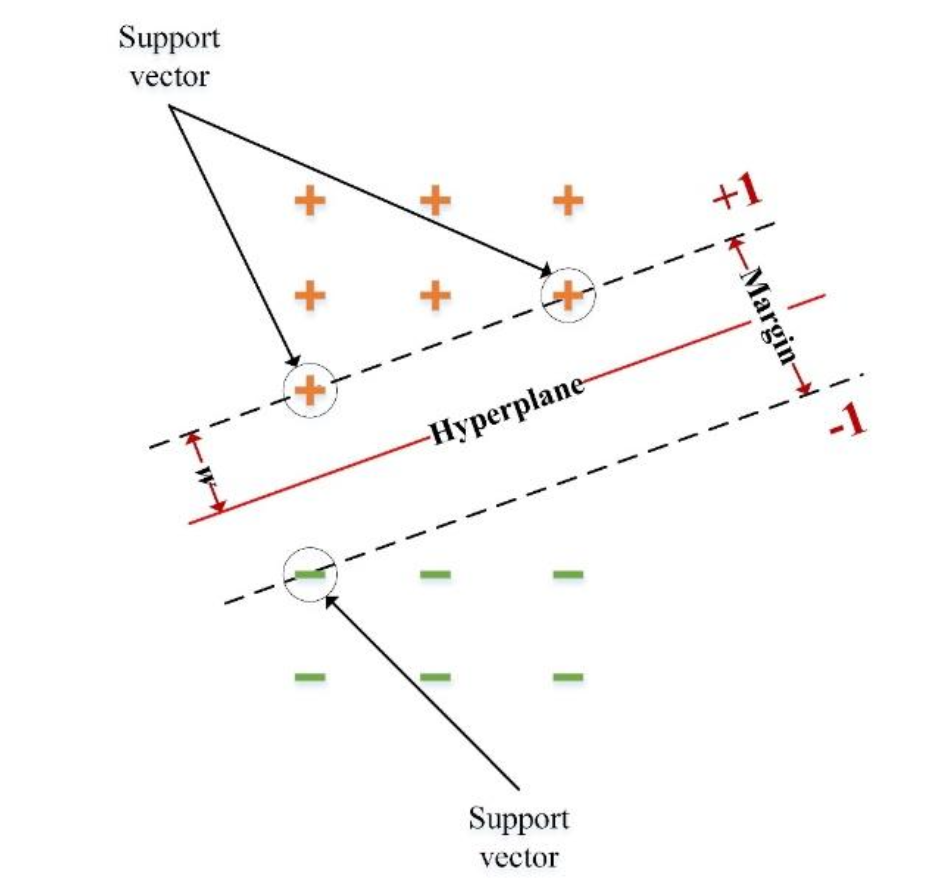
\includegraphics[width=0.55\textwidth]{figures/Classifiers/SVM.png}  
    \caption{An SVM hyperplane visually represents the maximum separation between the support vectors associated with the two classes, i.e., positive and negative \cite{jahed2020examining}. }
    \label{fig: SVM}
\end{figure*}
The Support Vector Machine (SVM) is a binary classification model that employ a hyperplane to classify two distinct data classes by optimizing the margin, which refers to the distance between the closest training instances from different classes \cite{survey_brain_biometrics}. SVMs are known for their strong generalization skills. What makes SVM particularly powerful is its emphasis on the points lying closest to the margin, called support vectors \cite{sahbi2019totally}. These support vectors play a pivotal role in defining the optimal hyperplane's position, allowing SVM to focus on the most informative instances and minimizing the influence of outliers \cite{pisner2020support}. This characteristic makes SVM inherently resistant to overfitting \cite{xia2015method}, ensuring that the model generalizes well to new, unseen data. Furthermore, SVM is not only limited to linear separations; it can also utilize kernel functions to transform the data into a higher-dimensional space \cite{pisner2020support}. This transformation can help SVM capture complex and nonlinear relationships between features, enabling it to handle intricate decision boundaries that may not be possible in the original feature space.
\smallskip

% The key strengths of SVM lie in its robustness, ability to handle high-dimensional data, and strong generalization capabilities. It excels in scenarios where the data is not only linearly separable but also when dealing with noisy or overlapping classes. SVM's optimization objective effectively minimizes the risk of misclassification by maximizing the margin, thereby promoting a clear distinction between the classes.
SVMs have been widely utilized in brainwave authentication research due to their ability to process intricate EEG data and effectively deliver precise subject identification.
Pham \textit{et al.} \cite{pham2013eeg} employed a SVM algorithm to analyze EEG data from a cohort of 9 participants actively involved in motor imagery activities. The researchers extracted key features from the EEG signals, specifically AR linear parameters and PSD components. The results showcased a remarkable performance with an EER spanning from 0$\%$ to 3.3$\%$.  

\subsection{Logistic Regression}
Logistic Regression is a statistical method used in machine learning for binary classification problems. It models the relationship between input features and the probability of a specific class using the logistic function, also known as the sigmoid function. The algorithm calculates a decision boundary that best separates the two classes based on the training data \cite{zabor2022logistic}. 
%Logistic Regression is a statistical method used in machine learning for binary classification problems. It models the relationship between input features and the probability of a specific class using the logistic function, also known as the sigmoid function. The algorithm calculates a decision boundary that best separates the two classes based on the training data.

\subsection{K Nearest Neighbour}
The K-Nearest Neighbour algorithm is a straightforward, non-parametric technique, implying that it arrives at decisions by considering the majority consensus of the nearest or most akin data points to the given inputs \cite{survey_brain_biometrics}. KNN operates through a two-step process. During the initial stage, it identifies the data points that are in close proximity to the target data point. The determination of closeness is accomplished via the use of distance metrics such as Euclidean or Manhattan distance. In the subsequent step, the algorithm assigns the target data point to a particular class based on the classes of its neighboring data points \cite{ghosh2023automatic}. Zúquete \textit{et al.} \cite{zuquete2010biometric} conducted a study that employed visual stimulation to elicit brain responses from 70 individuals, with the objective of biometric identification. By employing the KNN classifier, an average Area Under Curve (AUC) of 0.9817 was achieved, indicating strong performance in discriminating individuals based on their brain responses.  
%Brain responses were extracted with visual stimulation. The data set is composed of 70 individuals. With KNN classifier KNN, avg. AUC = 0.9817 was achieved. 

\subsection{Gaussian Naive Bayes}
The Naive Bayes (NB) theorem is a method rooted in probability theory, specifically Bayes' theorem, which elucidates the likelihood of a certain event occurring given prior knowledge about associated occurrences. Gaussian Naive Bayes is a specific variant of the Naive Bayes algorithm that assumes the features follow a Gaussian (normal) distribution \cite{jahromi2017non}. Put differently; it is assumed that the continuous values of attributes belonging to each class follow a normal distribution. This opposes the conventional assumption made by Naive Bayes that features are categorical and adhere to discrete distributions. Valsaraj \textit{et al.} \cite{valsaraj2020motor} conducted a comprehensive analysis of EEG signals to identify distinctive features associated with both physical movement and imagined upper limb motions. This research endeavor encompassed 10 participants and focused on four distinct upper limb movements. Employing the GNB algorithm for authentication purposes, the study achieved an impressive accuracy rate of 89$\%$ for imaginary motions and 85.7$\%$ for physical movement tasks. 

%Significantly, the conducted investigation produced remarkable outcomes, attaining an authentication accuracy rate of 89$\%$ for imaginary motions and 85.7$\%$ for physical movement, by employing the GNB algorithm. 
%Valsaraj \textit{et al.} \cite{valsaraj2020motor} presented study that analyzed the EEG signals for characteristic features elicited by movement and imagination of 4 different upper limb movements. The study involved 10 subjects. The signal was acquired using the EGI EEG headset (32 channels) with the Net Station toolbox. The study gave 89$\%$ accuracy achieved while utilizing Gaussian Naives Bayes algorithm for the authentication. 
\subsection{Random Forest}
The Random Forest (RF) algorithm, proposed by Breiman \cite{breiman2001random}, is a popular ensemble learning technique employed in machine learning to address classification and regression problems. It works by creating multiple decision trees during the training phase and then combines their predictions to make more accurate and robust predictions \cite{zhang2018new}. One key benefit of RF is its ability to handle high-dimensional feature spaces \cite{dm2020random}. EEG data frequently encompasses a substantial number of channels and temporal dimensions, leading to a considerable quantity of features. Random Forest's feature selection mechanism and ensemble approach allow it to effectively manage these complex feature sets, preventing overfitting and enhancing generalization \cite{dm2020random}. Another advantage is Random Forest's resilience to noisy data \cite{breiman2001random}. As previously mentioned in section \ref{sec:Background:Common EEG Artifacts}, it is important to acknowledge that EEG signals are prone to several artificats and sources of noise, which have the potential to impact the accuracy of categorization. RF ensemble approach mitigates this problem by averaging out the impact of noise, improving the overall robustness of the authentication system. RF has been employed in various EEG-based authentication works because of its adaptability to high-dimensional data, capability to handle complex relationships, and robustness against noise.
In the study conducted by Chowdhury and Imtiaz \cite{chowdhury2023machine}, EEG data was collected across three consecutive sessions, involving a total of 21 subjects. The research showcases that the proposed machine learning model, based on the random forest algorithm, demonstrates an authentication accuracy of approximately 83.2$\%$. 
%Chowdhury and Imtiaz \cite{chowdhury2023machine}. This data was collected over three sequential sessions involving 21 Subjects. The experiments show that the proposed random forest–based machine learning model can achieve approximately 83.2$\%$ authentication accuracy    

%Random Forest addresses overfitting and variance issues often found in individual decision trees. By averaging the predictions of multiple trees, it reduces the impact of outliers and noise in the data, leading to more stable and accurate results. Additionally, it provides a feature importance score, indicating which features contribute the most to the model's predictions. This can be valuable for understanding the importance of different variables in the dataset.
\subsection{Deep Learning}. 
%\end{itemize}
% \subsection{Common Performance Metrics}
% \begin{itemize}
%     \item Confusion metrics
%     \item Accuracy, Precision, Recall, F1-Score
%     \item EER
%     \item ROC-Curve
%     \item DET-Curve
%     \item FAR and FRR
% %\end{itemize}
\begin{table}[ht]
\caption{Authentication systems based on Brainwaves}
%\label{tab:Table 1}

\resizebox{\textwidth}{!}
    {
\begin{tabular}{l|ccclllll}

\hline

%Table column names
\rule{0pt}{25pt} \textbf{Paper} & \textbf{Year} & \textbf{$\#$Subjects} & \textbf{$\#$Channels} & \textbf{Data Acquisition} & \textbf{Features} & \textbf{Algorithm} & \textbf{Performance}\\
%\hline
%Data Acquistation Row
\hline
\rowcolor{Gray}
\rule{0pt}{25pt} Sun \cite{Sun_EEG_table_NN} & 2008 & 9 & 15 & Motor imagery & Energy & NN & \vtop{\hbox{\strut ACC: 92.52$\%$}\hbox{\strut ACC: 90.12$\%$}} \\

\rule{0pt}{25pt} Nakanishi et al. \cite{resting_state_related_work_3} & 2009 & 23 & 1  & Resting & \vtop{\hbox{\strut Fast Fourier}\hbox{\strut Trasnformation}\hbox{\strut (FFT)}} & \vtop{\hbox{\strut Convexity of}\hbox{\strut Spectral}\hbox{\strut distribution}} & ERR: 11\%$\\
\\

\rowcolor{Gray}
\rule{0pt}{25pt}Liwen et al. \cite{EEG_table_resting1} & 2010 & 40 & 1 & Resting & PSD & NBM & ERR: 4.16$\%$\\
\\

%ERP Devices Row
\vtop{\hbox{\strut Brighma and}\hbox{\strut Kumar \cite{EEG_table_motor_imagery_zotero}}} & 2010  & 6 & 128 & Motor imagery & AR & linear SVM & ACC: 99.76\%$  \\
\\

\rowcolor{Gray}
\rule{0pt}{25pt}Pham et al. \cite{EEG_table_motor1} & 2013 & 9 & 3 & Motor imagery & AR, PSD & SVM & ERR:  0-3.3$\%$ \\
\\

Rocca et al. \cite{la2013eeg} & 2013 & 36 & 3 & Resting & Bump Modelling & LDA & ACC: 99.69$\%$\\
\\

\rowcolor{Gray}
\rule{0pt}{25pt}Mu et al. \cite{EEG_table_EEG1} & 2016 & 10 & 2 & ERP & Fuzzy entropy & NN & \vtop{\hbox{\strut ACC: 87.3$\%$}\hbox{\strut FAR: 5.5$\%$}\hbox{\strut FRR: 5.6$\%$}} \\
\\

\vtop{\hbox{\strut Abo-Zahhad}\hbox{\strut et al. \cite{brainwaves_as_biometric}}} & 2016 & 31 & 1 & \vtop{\hbox{\strut Eye blink, Resting}\hbox{\strut ERP}} & AR & LDA & \vtop{\hbox{\strut ACC: 99.68$\%$}\hbox{\strut EER: 0.89-4.4$\%$}} \\
\\
\rowcolor{Gray}
\rule{0pt}{25pt} Huang et al. \cite{huang2019eeg} & 2019 & 30 & 14 & ERP & \vtop{\hbox{\strut Maximum}\hbox{\strut Entropy}\hbox{\strut Skewness}\hbox{\strut Standard Deviation (SD)}} & \vtop{\hbox{\strut NB, NN}\hbox{\strut LR}} & \vtop{\hbox{\strut ACC: 80.74$\%$}\hbox{\strut True Positive Rate (TPR): 78.90$\%$}\hbox{\strut False Positive Rate (FPR): 17.41$\%$}}\\
\\

\vtop{\hbox{\strut Puengdang}\hbox{\strut et al. \cite{ERP_Table_puengdang2019eeg}}} & 2019 & 20 & 18 & ERP & N.A. & NN & \vtop{\hbox{\strut FAR: 6.58$\%$}\hbox{\strut FRR: 10.53$\%$}} \\
\\
\rowcolor{Gray}
\rule{0pt}{25pt}Zeng et al. \cite{ERP_table_zeng2018eeg} & 2019 & 22 & 16 & ERP & \vtop{\hbox{\strut Fisher Linear}\hbox{\strut Discriminant (FLD)}\hbox{\strut analysis}} & \vtop{\hbox{\strut Hierarchical Discriminant}\hbox{\strut  Component Analysis}\hbox{\strut (HDCA)}} & \vtop{\hbox{\strut ACC: 94.26$\%$}\hbox{\strut FAR: 6.27$\%$}\hbox{\strut FRR: 5.26$\%$}}\\
\\

%ERP Devices Row
Yu et al. \cite{ERP_table_yu2019eeg} & 2020 & 8 & 9 & ERP & N.A. & NN & \vtop{\hbox{\strut ACC: 96.78$\%$}\hbox{\strut FAR: 0.06$\%$}\hbox{\strut FRR: 3.15$\%$}} \\
\\

\rowcolor{Gray}
\rule{0pt}{25pt}\vtop{\hbox{\strut Sooriyaarachchi}\hbox{\strut et al. \cite{sooriyaarachchi2020musicid}}} & 2021 & 20 & 4 & ERP & \vtop{\hbox{\strut Maximum}\hbox{\strut Minimum}\hbox{\strut Mean}\hbox{\strut Zero Crossing Rate (ZCS)}} & Random Forest (RF) & ACC: 97$\%$\\

\hline
\end{tabular}
}
\end{table}
